% 3.In your report, answer the following questions.

% A. Visualize 3D points with the “MeshLab” program

% B. [BONUS 1] Analyze the difference in reconstruction results as each method changes.
% i. Feature extraction methods, feature matching methods, RANSAC variants,
% distance measures etc.. (Related to assignment 9)

% C. [BONUS 2] Take two images directly and perform 3D reconstruction.
% i. Estimate intrinsic parameters through camera calibration. (Related to
% assignment 8)

\section{Implementation}

The implementation uses the fundamental matrix estimation code from assigment
9. However, because my estimation had some very big errors in it, I had to
rewrite that code. It should work okay now.

Other than that the code is mostly just following the steps laid out in the
assigment. In the triangulation I opted for a simple linear estimation, which
seems to work well enough, in this case at least. Not even normalization was
needed.


\section{Analysis}

A RANSAC distance threshold of 10 was found to produce good results. With it,
it found the \(\approx1030\) inliers quite fast, within 300 iterations or so.
Additional iterations didn't produce more inliers.

Opposed to previous RANSAC assignments, this time the results were really
stable. Different runs didn't produce noticeably different results.


\section{Results}

The following figures have the resulting point cloud. It is impressively good,
considering how much trouble I have had with the fundamental matrix estimation.

\begin{figure}[h]
  \centering
  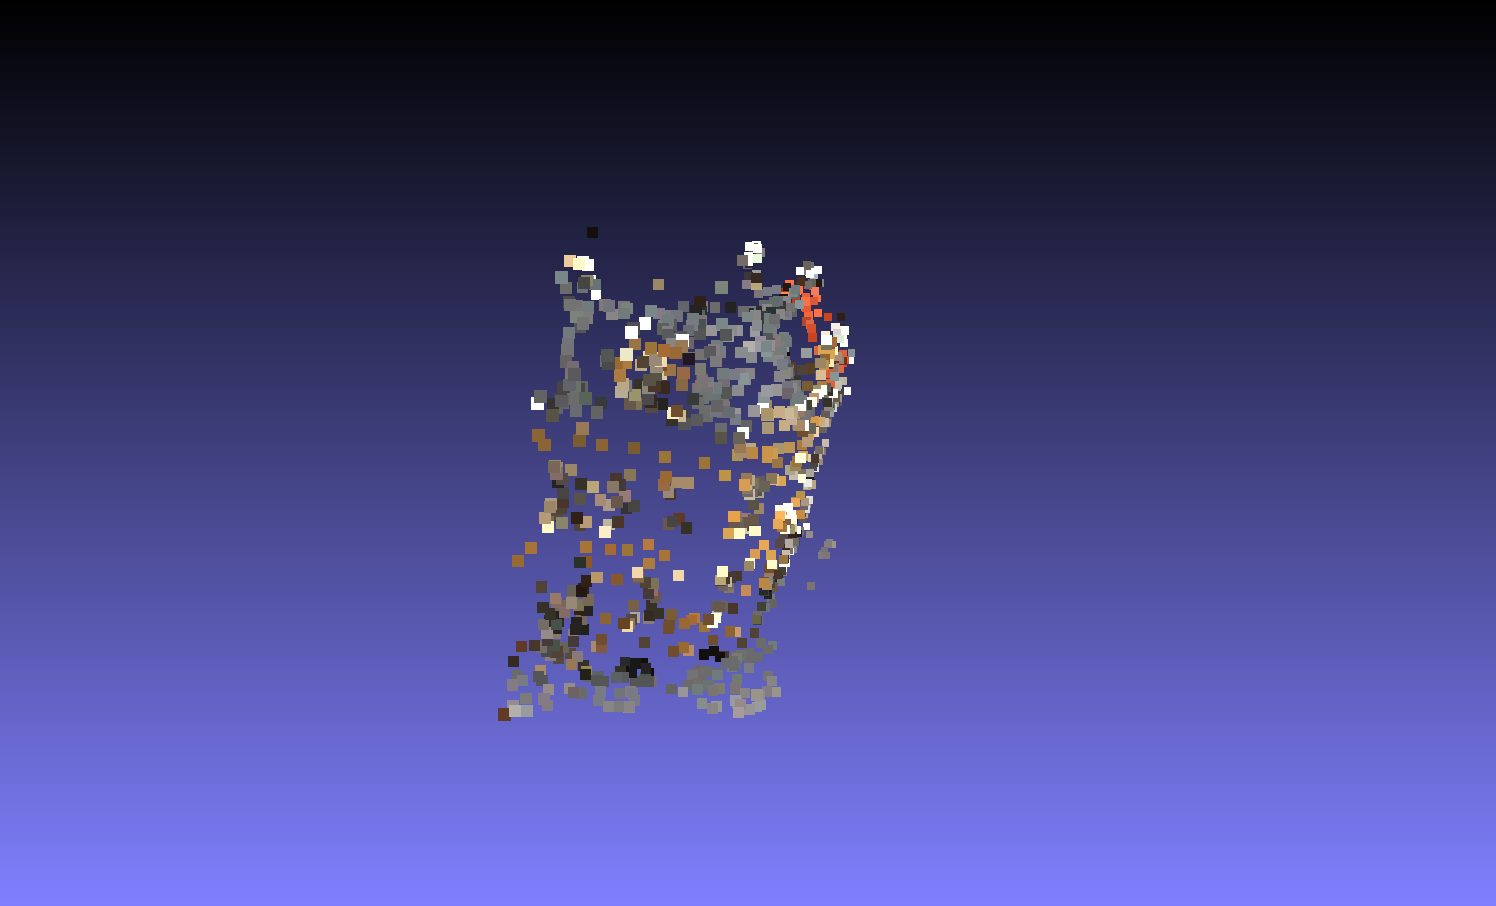
\includegraphics[width=0.8\linewidth]{snapshot00}
\end{figure}

\begin{figure}[h]
  \centering
  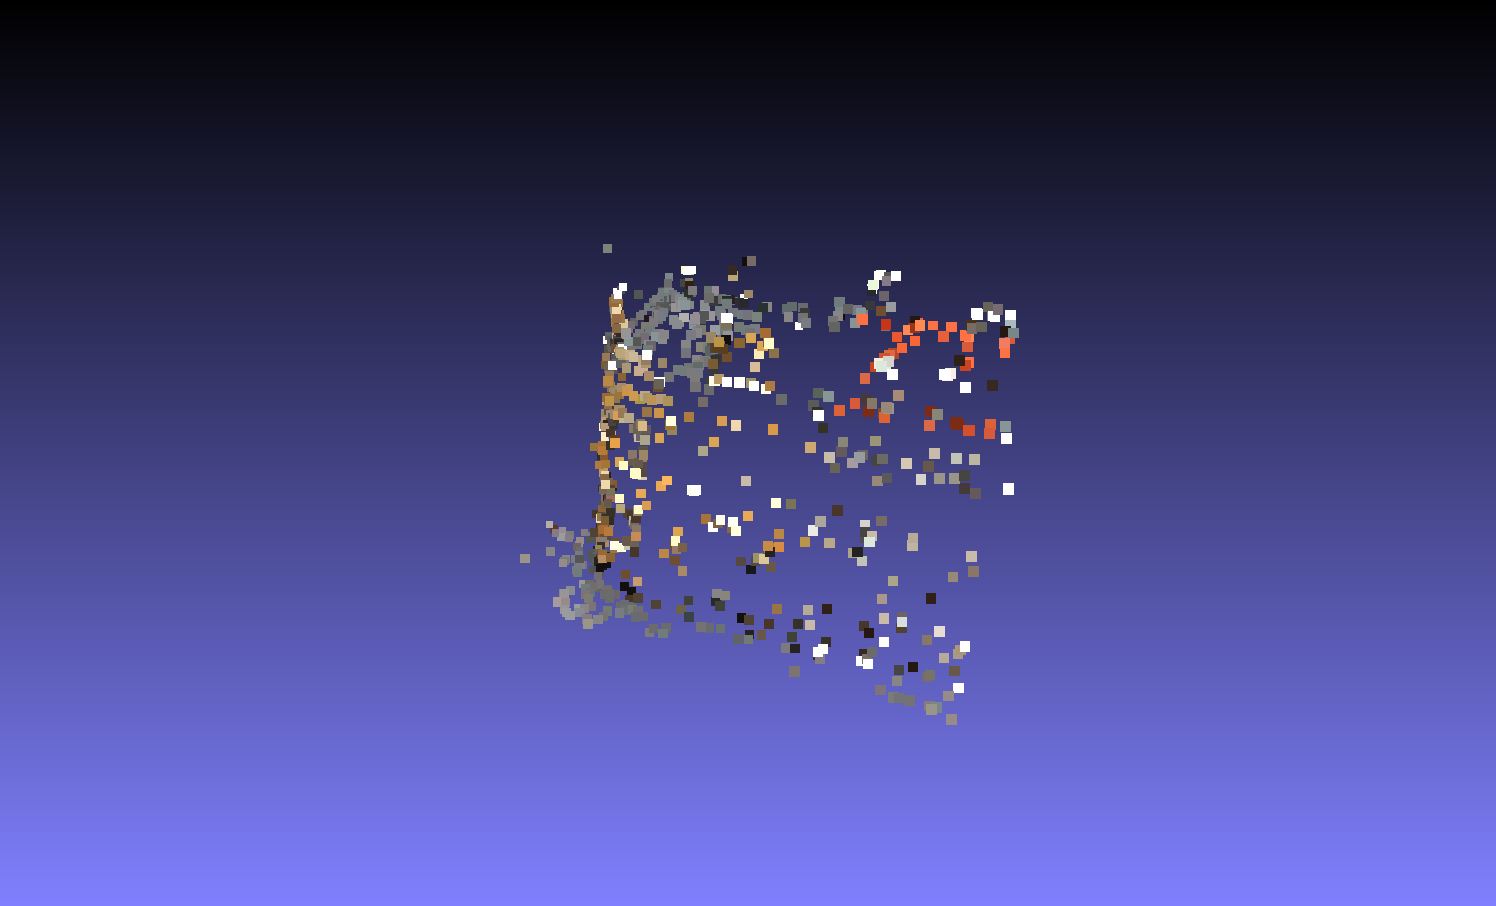
\includegraphics[width=0.8\linewidth]{snapshot01}
\end{figure}

\begin{figure}[h]
  \centering
  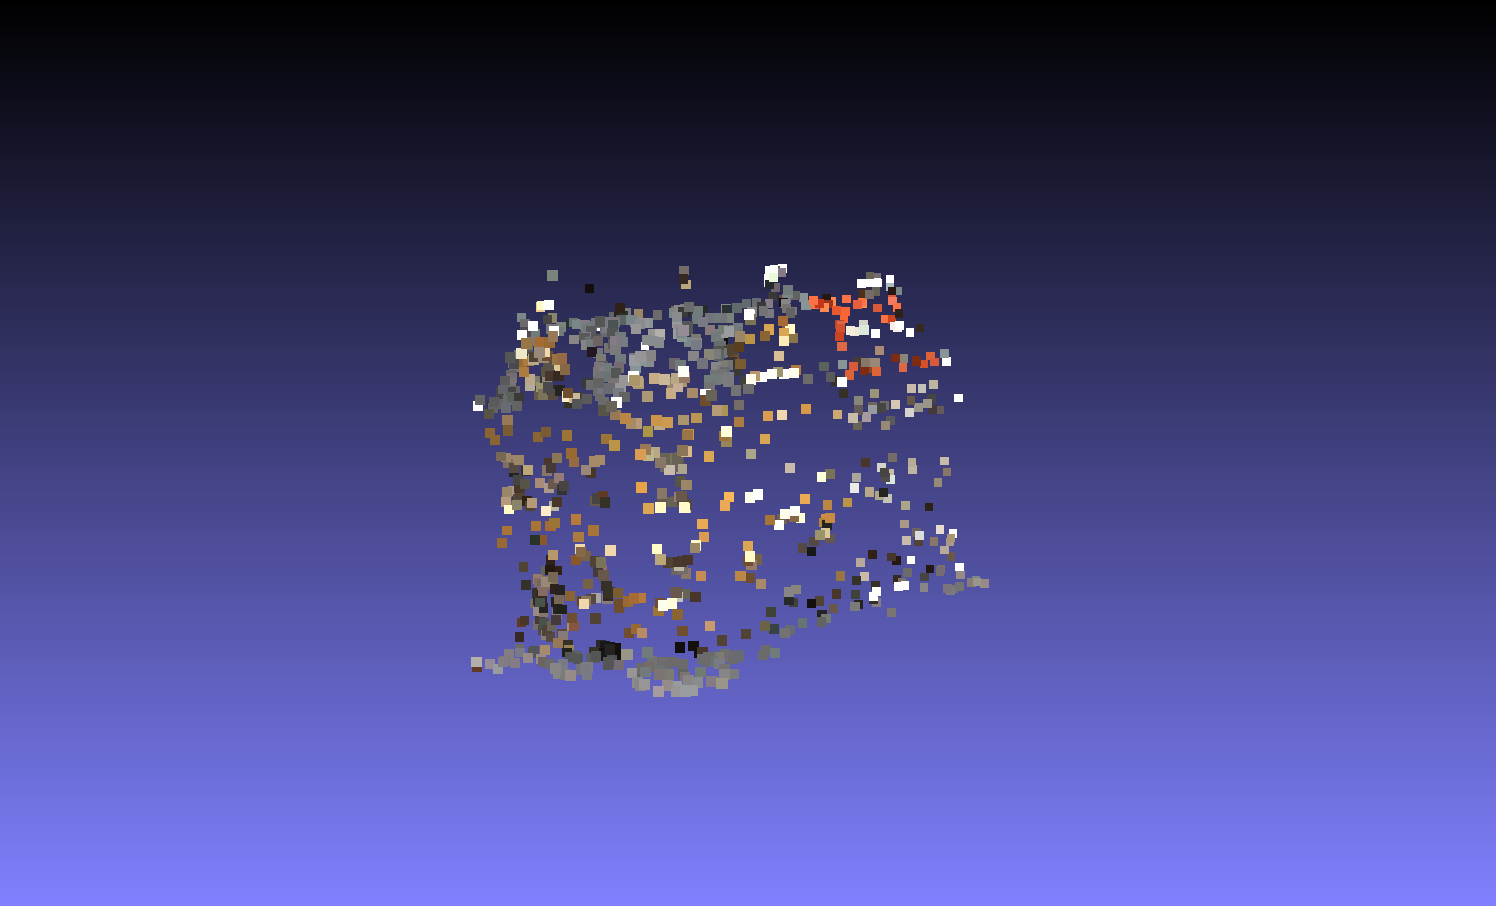
\includegraphics[width=0.8\linewidth]{snapshot02}
\end{figure}

\begin{figure}[h]
  \centering
  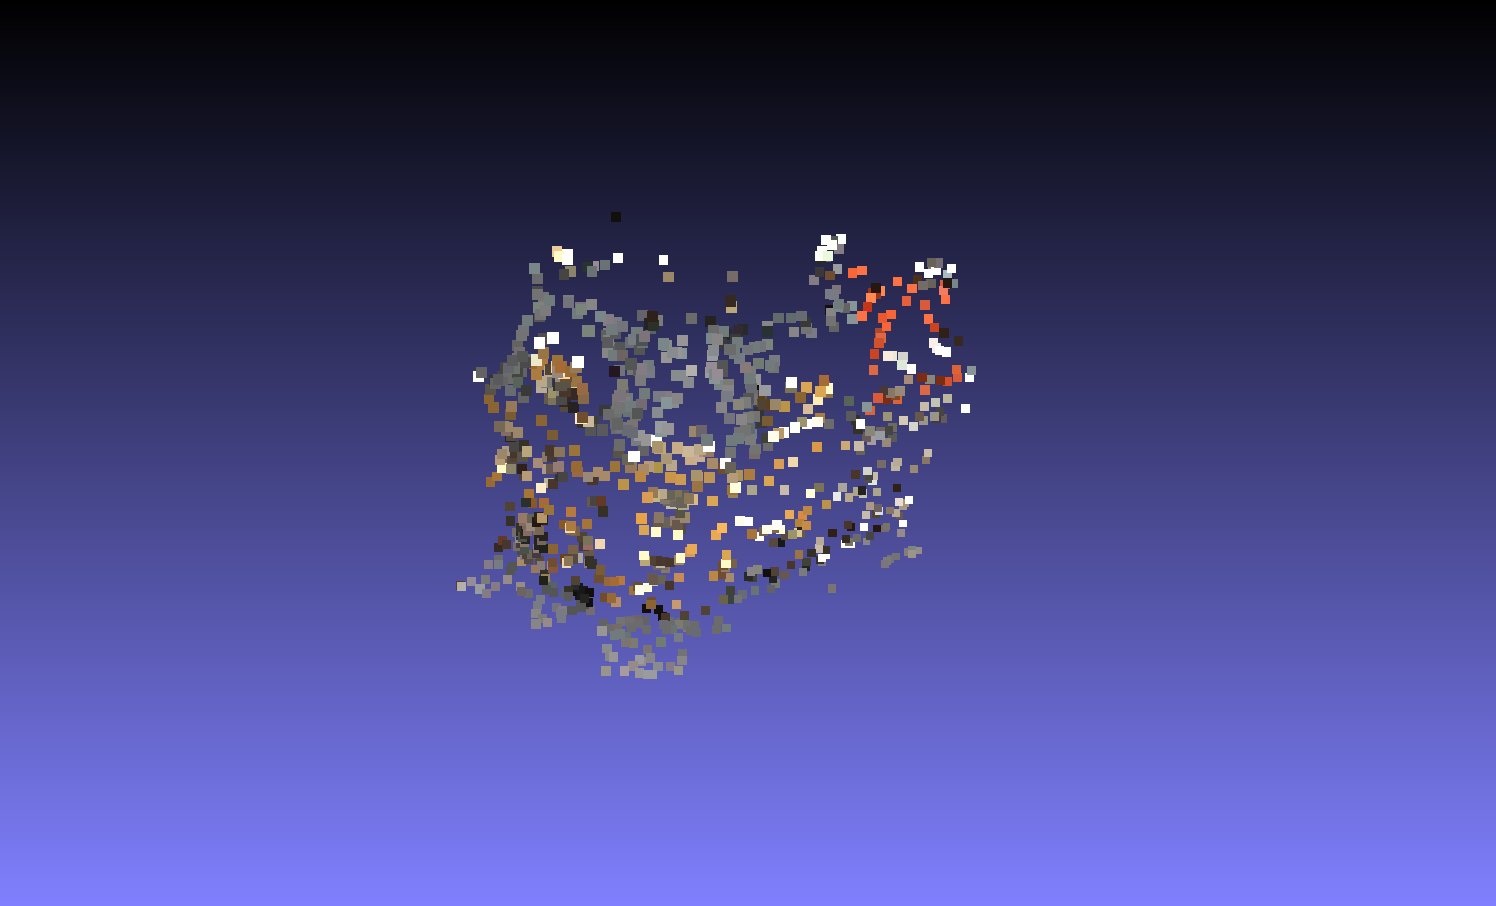
\includegraphics[width=0.8\linewidth]{snapshot03}
\end{figure}

\begin{figure}[h]
  \centering
  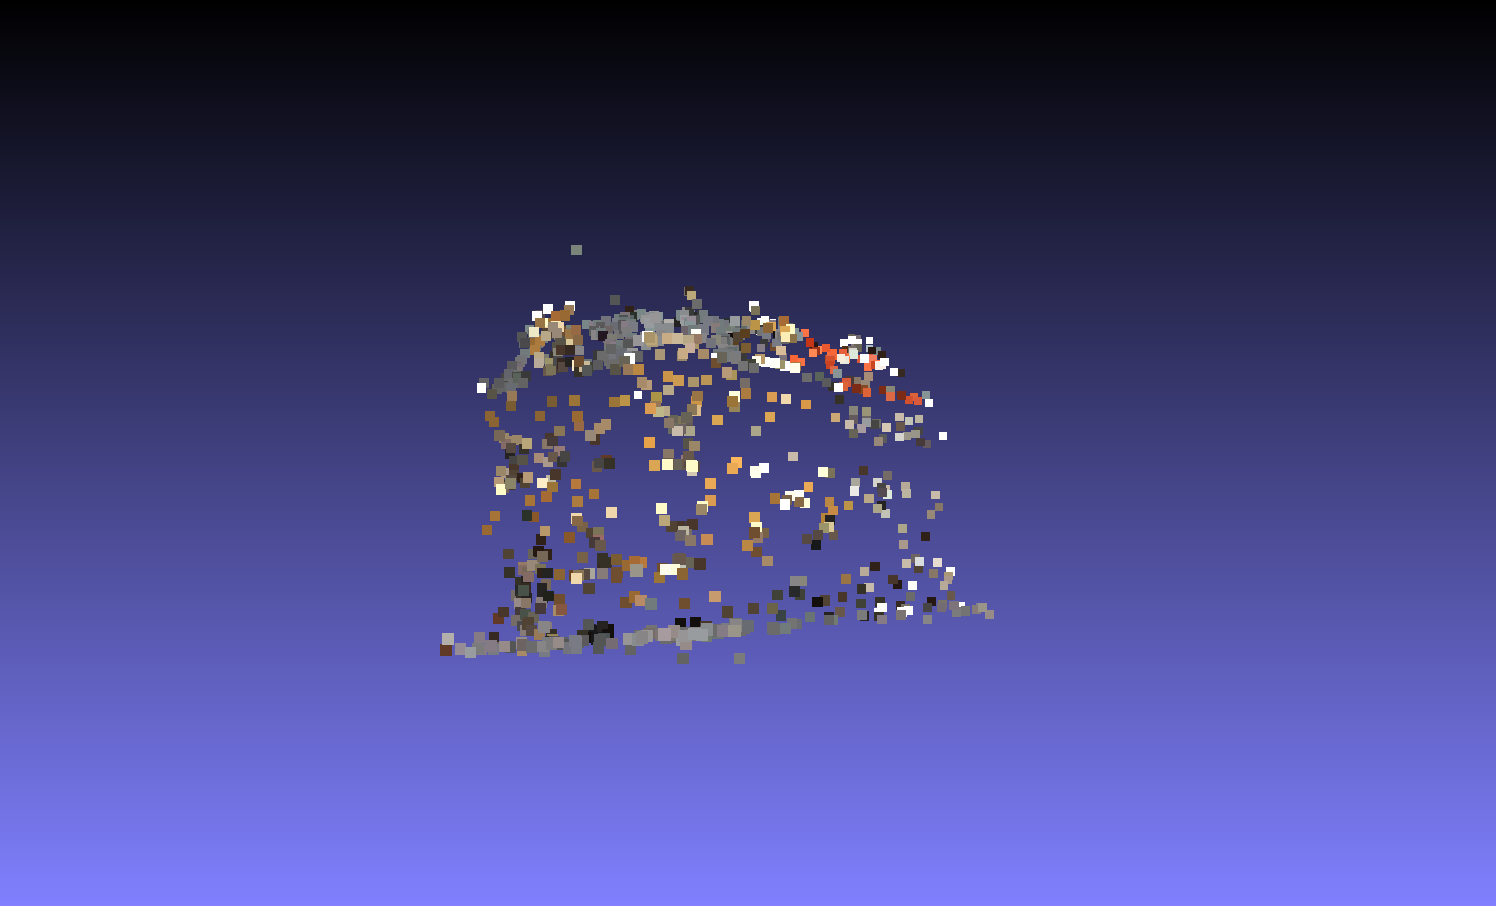
\includegraphics[width=0.8\linewidth]{snapshot04}
\end{figure}
